\documentclass[12pt]{article}

\usepackage{sbc-template}
\usepackage{graphicx,url}
\usepackage[utf8]{inputenc}
\usepackage[brazil]{babel}
\usepackage[latin1]{inputenc}  

     
\sloppy

\title{Plataforma de monitoramento e diagnóstico clínico de arbovírus utilizando modelos computacionais}

% \author{Luciana P. Nedel\inst{1}, Rafael H. Bordini\inst{2}, Flávio Rech
%   Wagner\inst{1}, Jomi F. Hübner\inst{3} }


% \address{Instituto de Informática -- Universidade Federal do Rio Grande do Sul
%   (UFRGS)\\
%   Caixa Postal 15.064 -- 91.501-970 -- Porto Alegre -- RS -- Brazil
% \nextinstitute
%   Department of Computer Science -- University of Durham\\
%   Durham, U.K.
% \nextinstitute
%   Departamento de Sistemas e Computação\\
%   Universidade Regional de Blumenal (FURB) -- Blumenau, SC -- Brazil
%   \email{\{nedel,flavio\}@inf.ufrgs.br, R.Bordini@durham.ac.uk,
%   jomi@inf.furb.br}
% }

\begin{document} 

\maketitle

% \begin{abstract}
%   This meta-paper describes the style to be used in articles and short papers
%   for SBC conferences. For papers in English, you should add just an abstract
%   while for the papers in Portuguese, we also ask for an abstract in
%   Portuguese (``resumo''). In both cases, abstracts should not have more than
%   10 lines and must be in the first page of the paper.
% \end{abstract}
     
% \begin{resumo} 
%   Este meta-artigo descreve o estilo a ser usado na confecção de artigos e
%   resumos de artigos para publicação nos anais das conferências organizadas
%   pela SBC. É solicitada a escrita de resumo e abstract apenas para os artigos
%   escritos em português. Artigos em inglês deverão apresentar apenas abstract.
%   Nos dois casos, o autor deve tomar cuidado para que o resumo (e o abstract)
%   não ultrapassem 10 linhas cada, sendo que ambos devem estar na primeira
%   página do artigo.
% \end{resumo}


\section{Introdução}

Segundo a Organização Mundial da Saúde (OMS), em continentes tropicais como Ásia, África e América, cerca de um bilhão de pessoas são infectadas por doenças transmitidas por vetores (organismos que transmitem doenças infecciosas) anualmente \cite{PAPER04}, \cite{PAPER01}. Na maioria dos casos, esses vetores são mosquitos; e dentre eles destacam-se o \textit{Aedes aegypti} e o \textit{Aedes albopictus}. Ambos são vetores para doenças arbovirais como: Dengue (DENV), Chikungunya (CHIKV), Zika (ZIKV) e Febre amarela.

As doenças arbovirais mencionadas têm se tornando um problema de saúde global devido à sua rápida disseminação geográfica \cite{PAPER01}, por conta das mudanças climáticas, desmatamentos, migração populacional, ocupação desordenada de áreas urbanas, precariedade das condições sanitárias \cite{PAPER05}. Nos últimos 30 anos, o impacto na saúde pública desses arbovírus aumentou dramaticamente \cite{PAPER01}. Cerca de 86\% de 250 nações/territórios no mundo, apresentam condições favoráveis para a instalação e a proliferação dos mosquitos transmissores dessas doenças \cite{PAPER01}.

De acordo com a Organização Pan-Americana de Saúde (APAS), só o Brasil corresponde a mais de 70\% dos 2,8 milhões de casos confirmados de DENV em 2019 [2]. Além disso, a CHIKV corresponde a 110.627 e a ZIKV com 9.813 casos prováveis [6]. O impacto dessas doenças foi suficiente para estabelecer situação de emergência em saúde pública pelo Ministério da Saúde e pela OMS no país. Isso implicou na mobilização de recursos e articulações entre estados e municípios para enfrentamento da circulação do vírus, a investigação epidemiológica deve fazer parte da vigilância epidemiológica e das preocupações da saúde pública nacional \cite{PAPER07}.

Apesar do aumento expressivo de casos no mundo da DENV, CHIKV e ZIKV ainda há dificuldade na identificação a partir dos sintomas por conta de sua similaridade \cite{PAPER03}. São essenciais esforços para o desenvolvimento e aperfeiçoamento de exames diagnósticos \cite{PAPER07}. Nesse contexto, têm se tornado cada vez mais comum o uso de técnicas de aprendizado de máquina e de mineração de dados para diagnóstico e prognóstico dessas  doenças \cite{PAPER03}. 

Alguns trabalhos na literatura \cite{PAPER08}, \cite{PAPER09} e \cite{PAPER10}, têm adotado essas técnicas para classificação, buscando identificar mosquitos (\textit{Aedes aegypti} e outros) e possíveis áreas de proliferação através de processamento de imagens para detecção de foco de transmissão da doença. Outros trabalhos têm concentrado suas pesquisas no diagnóstico desses arbovírus \cite{PAPER11}, \cite{PAPER12} e \cite{PAPER13}, em sua maioria analisam os principais sintomas e exames laboratoriais a fim reduzir a incidência e a mortalidade e prevenir epidemias causadas por doenças transmitidas por esses vetores. A aplicação de técnicas computacionais para prognóstico dessas doenças é essencial para descobrir padrões de diagnóstico para prever os pacientes infectados com vírus e seus possíveis resultados.

Diante dos desafios e limitações operacionais relacionados à confirmação diagnóstica no Brasil, o desenvolvimento de modelos computacionais para monitoramento e classificação diagnóstica com base em dados clínicos, sintomas e exames laboratoriais apresenta-se como solução de baixo custo que pode contribuir para melhorar o registro preciso de casos confirmados de DENV, CHIKV, ZIKV e outros arbovírus. Para tanto, este trabalho propõe uma plataforma para monitoramento e diagnóstico clínico de arbovírus usando modelos de machine learning. Existem três módulos principais: suporte à decisão, monitoramento e interface gráfica. 

O módulo de apoio à decisão utiliza os dados disponíveis nos bancos de dados de saúde brasileiros, como o Sistema de Informação de Agravos de Notificação (SINAN), que contém dados de pacientes com doenças de notificação obrigatória, e o Sistema de Informação sobre Mortalidade (SIM), que contém dados de mortalidade. Modelos de deep learning são propostos para a classificação e previsão de epidemias de arbovírus. A seleção de preditores deve ser orientada e validada por um profissional de saúde para evitar possíveis vieses nos resultados. Da mesma forma, antes da proposta dos modelos de aprendizado de máquina, é necessária a execução de uma Análise Exploratória de Dados (EDA) dos dados históricos para identificar padrões e, assim, auxiliar na seleção dos métodos mais adequados. 

O módulo de monitoramento irá monitorar os dados dos bancos de dados disponíveis e gerará entradas para a interface gráfica, como alertas de epidemias. Com os resultados deste trabalho, pretende-se melhorar a capacidade de classificação dos diferentes arbovírus existentes no Brasil, contribuindo para uma melhor vigilância entomológica e epidemiológica, controle de vetores e mitigação de doenças, gerenciamento clínico mais eficaz e tratamento do paciente e recuperação mais eficiente de dados em tempo hábil. A tecnologia resultante, tanto do ponto de vista do laboratório quanto da análise, pode ser transferida para o hospital geral e pode ser aplicada como parte das atividades gerais de vigilância em saúde, contribuindo para o Sistema Único de Saúde (SUS).

% \section{Proposta} \label{sec:firstpage}



% \section{CD-ROMs and Printed Proceedings}

% In some conferences, the papers are published on CD-ROM while only the
% abstract is published in the printed Proceedings. In this case, authors are
% invited to prepare two final versions of the paper. One, complete, to be
% published on the CD and the other, containing only the first page, with
% abstract and ``resumo'' (for papers in Portuguese).

% \section{Sections and Paragraphs}

% Section titles must be in boldface, 13pt, flush left. There should be an extra
% 12 pt of space before each title. Section numbering is optional. The first
% paragraph of each section should not be indented, while the first lines of
% subsequent paragraphs should be indented by 1.27 cm.

% \subsection{Subsections}

% The subsection titles must be in boldface, 12pt, flush left.

% \section{Figures and Captions}\label{sec:figs}


% Figure and table captions should be centered if less than one line
% (Figure~\ref{fig:exampleFig1}), otherwise justified and indented by 0.8cm on
% both margins, as shown in Figure~\ref{fig:exampleFig2}. The caption font must
% be Helvetica, 10 point, boldface, with 6 points of space before and after each
% caption.

% \begin{figure}[ht]
% \centering
% 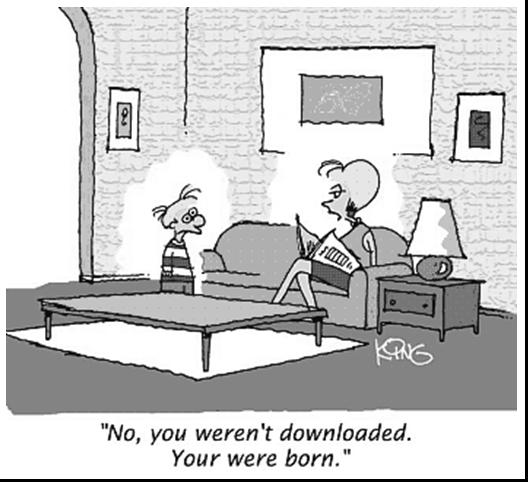
\includegraphics[width=.5\textwidth]{fig1.jpg}
% \caption{A typical figure}
% \label{fig:exampleFig1}
% \end{figure}

% \begin{figure}[ht]
% \centering
% 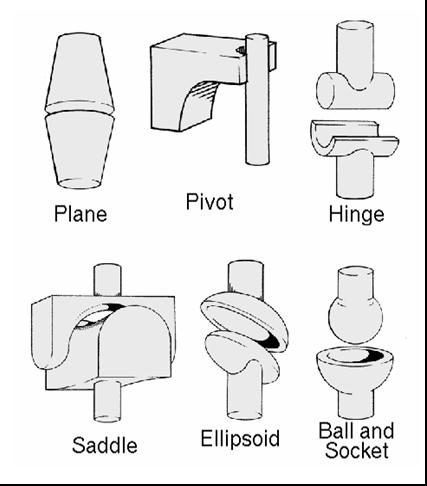
\includegraphics[width=.3\textwidth]{fig2.jpg}
% \caption{This figure is an example of a figure caption taking more than one
%   line and justified considering margins mentioned in Section~\ref{sec:figs}.}
% \label{fig:exampleFig2}
% \end{figure}

% In tables, try to avoid the use of colored or shaded backgrounds, and avoid
% thick, doubled, or unnecessary framing lines. When reporting empirical data,
% do not use more decimal digits than warranted by their precision and
% reproducibility. Table caption must be placed before the table (see Table 1)
% and the font used must also be Helvetica, 10 point, boldface, with 6 points of
% space before and after each caption.

% \begin{table}[ht]
% \centering
% \caption{Variables to be considered on the evaluation of interaction
%   techniques}
% \label{tab:exTable1}
% 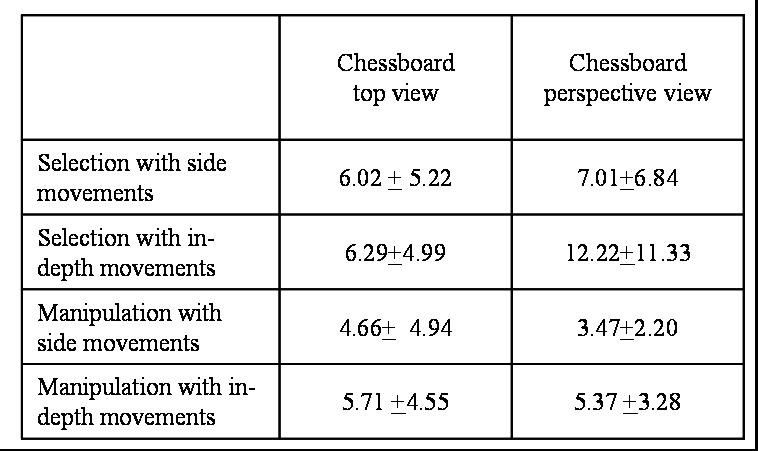
\includegraphics[width=.7\textwidth]{table.jpg}
% \end{table}

% \section{Images}

% All images and illustrations should be in black-and-white, or gray tones,
% excepting for the papers that will be electronically available (on CD-ROMs,
% internet, etc.). The image resolution on paper should be about 600 dpi for
% black-and-white images, and 150-300 dpi for grayscale images.  Do not include
% images with excessive resolution, as they may take hours to print, without any
% visible difference in the result. 

% \section{References}

% Bibliographic references must be unambiguous and uniform.  We recommend giving
% the author names references in brackets, e.g. \cite{knuth:84},
% \cite{boulic:91}, and \cite{smith:99}.

% The references must be listed using 12 point font size, with 6 points of space
% before each reference. The first line of each reference should not be
% indented, while the subsequent should be indented by 0.5 cm.

\bibliographystyle{sbc}
\bibliography{sbc-template}

\end{document}
